% Options for packages loaded elsewhere
\PassOptionsToPackage{unicode}{hyperref}
\PassOptionsToPackage{hyphens}{url}
%
\documentclass[
]{article}
\usepackage{lmodern}
\usepackage{amssymb,amsmath}
\usepackage{ifxetex,ifluatex}
\ifnum 0\ifxetex 1\fi\ifluatex 1\fi=0 % if pdftex
  \usepackage[T1]{fontenc}
  \usepackage[utf8]{inputenc}
  \usepackage{textcomp} % provide euro and other symbols
\else % if luatex or xetex
  \usepackage{unicode-math}
  \defaultfontfeatures{Scale=MatchLowercase}
  \defaultfontfeatures[\rmfamily]{Ligatures=TeX,Scale=1}
\fi
% Use upquote if available, for straight quotes in verbatim environments
\IfFileExists{upquote.sty}{\usepackage{upquote}}{}
\IfFileExists{microtype.sty}{% use microtype if available
  \usepackage[]{microtype}
  \UseMicrotypeSet[protrusion]{basicmath} % disable protrusion for tt fonts
}{}
\makeatletter
\@ifundefined{KOMAClassName}{% if non-KOMA class
  \IfFileExists{parskip.sty}{%
    \usepackage{parskip}
  }{% else
    \setlength{\parindent}{0pt}
    \setlength{\parskip}{6pt plus 2pt minus 1pt}}
}{% if KOMA class
  \KOMAoptions{parskip=half}}
\makeatother
\usepackage{xcolor}
\IfFileExists{xurl.sty}{\usepackage{xurl}}{} % add URL line breaks if available
\IfFileExists{bookmark.sty}{\usepackage{bookmark}}{\usepackage{hyperref}}
\hypersetup{
  pdftitle={Exploring the On-demand Video Streaming Industry and Looking for a Niche Untapped Market},
  pdfauthor={Ali Mir \& Johanna Wameling},
  hidelinks,
  pdfcreator={LaTeX via pandoc}}
\urlstyle{same} % disable monospaced font for URLs
\usepackage[margin=1in]{geometry}
\usepackage{color}
\usepackage{fancyvrb}
\newcommand{\VerbBar}{|}
\newcommand{\VERB}{\Verb[commandchars=\\\{\}]}
\DefineVerbatimEnvironment{Highlighting}{Verbatim}{commandchars=\\\{\}}
% Add ',fontsize=\small' for more characters per line
\usepackage{framed}
\definecolor{shadecolor}{RGB}{248,248,248}
\newenvironment{Shaded}{\begin{snugshade}}{\end{snugshade}}
\newcommand{\AlertTok}[1]{\textcolor[rgb]{0.94,0.16,0.16}{#1}}
\newcommand{\AnnotationTok}[1]{\textcolor[rgb]{0.56,0.35,0.01}{\textbf{\textit{#1}}}}
\newcommand{\AttributeTok}[1]{\textcolor[rgb]{0.77,0.63,0.00}{#1}}
\newcommand{\BaseNTok}[1]{\textcolor[rgb]{0.00,0.00,0.81}{#1}}
\newcommand{\BuiltInTok}[1]{#1}
\newcommand{\CharTok}[1]{\textcolor[rgb]{0.31,0.60,0.02}{#1}}
\newcommand{\CommentTok}[1]{\textcolor[rgb]{0.56,0.35,0.01}{\textit{#1}}}
\newcommand{\CommentVarTok}[1]{\textcolor[rgb]{0.56,0.35,0.01}{\textbf{\textit{#1}}}}
\newcommand{\ConstantTok}[1]{\textcolor[rgb]{0.00,0.00,0.00}{#1}}
\newcommand{\ControlFlowTok}[1]{\textcolor[rgb]{0.13,0.29,0.53}{\textbf{#1}}}
\newcommand{\DataTypeTok}[1]{\textcolor[rgb]{0.13,0.29,0.53}{#1}}
\newcommand{\DecValTok}[1]{\textcolor[rgb]{0.00,0.00,0.81}{#1}}
\newcommand{\DocumentationTok}[1]{\textcolor[rgb]{0.56,0.35,0.01}{\textbf{\textit{#1}}}}
\newcommand{\ErrorTok}[1]{\textcolor[rgb]{0.64,0.00,0.00}{\textbf{#1}}}
\newcommand{\ExtensionTok}[1]{#1}
\newcommand{\FloatTok}[1]{\textcolor[rgb]{0.00,0.00,0.81}{#1}}
\newcommand{\FunctionTok}[1]{\textcolor[rgb]{0.00,0.00,0.00}{#1}}
\newcommand{\ImportTok}[1]{#1}
\newcommand{\InformationTok}[1]{\textcolor[rgb]{0.56,0.35,0.01}{\textbf{\textit{#1}}}}
\newcommand{\KeywordTok}[1]{\textcolor[rgb]{0.13,0.29,0.53}{\textbf{#1}}}
\newcommand{\NormalTok}[1]{#1}
\newcommand{\OperatorTok}[1]{\textcolor[rgb]{0.81,0.36,0.00}{\textbf{#1}}}
\newcommand{\OtherTok}[1]{\textcolor[rgb]{0.56,0.35,0.01}{#1}}
\newcommand{\PreprocessorTok}[1]{\textcolor[rgb]{0.56,0.35,0.01}{\textit{#1}}}
\newcommand{\RegionMarkerTok}[1]{#1}
\newcommand{\SpecialCharTok}[1]{\textcolor[rgb]{0.00,0.00,0.00}{#1}}
\newcommand{\SpecialStringTok}[1]{\textcolor[rgb]{0.31,0.60,0.02}{#1}}
\newcommand{\StringTok}[1]{\textcolor[rgb]{0.31,0.60,0.02}{#1}}
\newcommand{\VariableTok}[1]{\textcolor[rgb]{0.00,0.00,0.00}{#1}}
\newcommand{\VerbatimStringTok}[1]{\textcolor[rgb]{0.31,0.60,0.02}{#1}}
\newcommand{\WarningTok}[1]{\textcolor[rgb]{0.56,0.35,0.01}{\textbf{\textit{#1}}}}
\usepackage{graphicx}
\makeatletter
\def\maxwidth{\ifdim\Gin@nat@width>\linewidth\linewidth\else\Gin@nat@width\fi}
\def\maxheight{\ifdim\Gin@nat@height>\textheight\textheight\else\Gin@nat@height\fi}
\makeatother
% Scale images if necessary, so that they will not overflow the page
% margins by default, and it is still possible to overwrite the defaults
% using explicit options in \includegraphics[width, height, ...]{}
\setkeys{Gin}{width=\maxwidth,height=\maxheight,keepaspectratio}
% Set default figure placement to htbp
\makeatletter
\def\fps@figure{htbp}
\makeatother
\setlength{\emergencystretch}{3em} % prevent overfull lines
\providecommand{\tightlist}{%
  \setlength{\itemsep}{0pt}\setlength{\parskip}{0pt}}
\setcounter{secnumdepth}{-\maxdimen} % remove section numbering
\ifluatex
  \usepackage{selnolig}  % disable illegal ligatures
\fi

\title{Exploring the On-demand Video Streaming Industry and Looking for
a Niche Untapped Market}
\usepackage{etoolbox}
\makeatletter
\providecommand{\subtitle}[1]{% add subtitle to \maketitle
  \apptocmd{\@title}{\par {\large #1 \par}}{}{}
}
\makeatother
\subtitle{R for Data Science @ Hult International Business School}
\author{Ali Mir \& Johanna Wameling}
\date{12/21/2020}

\begin{document}
\maketitle

{
\setcounter{tocdepth}{2}
\tableofcontents
}
\begin{center}\rule{0.5\linewidth}{0.5pt}\end{center}

\hypertarget{framing-the-problem}{%
\section{Framing the Problem}\label{framing-the-problem}}

\begin{center}\rule{0.5\linewidth}{0.5pt}\end{center}

\hypertarget{problem-recognition}{%
\subsection{Problem Recognition}\label{problem-recognition}}

\begin{center}\rule{0.5\linewidth}{0.5pt}\end{center}

The on-demand video streaming industry is experiencing exponential
growth in recent years and more players are entering the market (Ibis
World, 2020). The following analysis looks into the volume of content
per platform, the quality, according to ratings and other
characteristics as a means to compare the four leading streaming
providers' content. As the industry is expected to grow around 20\% YoY
for the next five years, this competitive analysis aims to shed light on
the existing competition and positioning of the players to find a
potential niche opening for new entrants.

\begin{center}\rule{0.5\linewidth}{0.5pt}\end{center}

\hypertarget{review-of-previous-findings}{%
\subsection{Review of Previous
Findings}\label{review-of-previous-findings}}

\begin{center}\rule{0.5\linewidth}{0.5pt}\end{center}

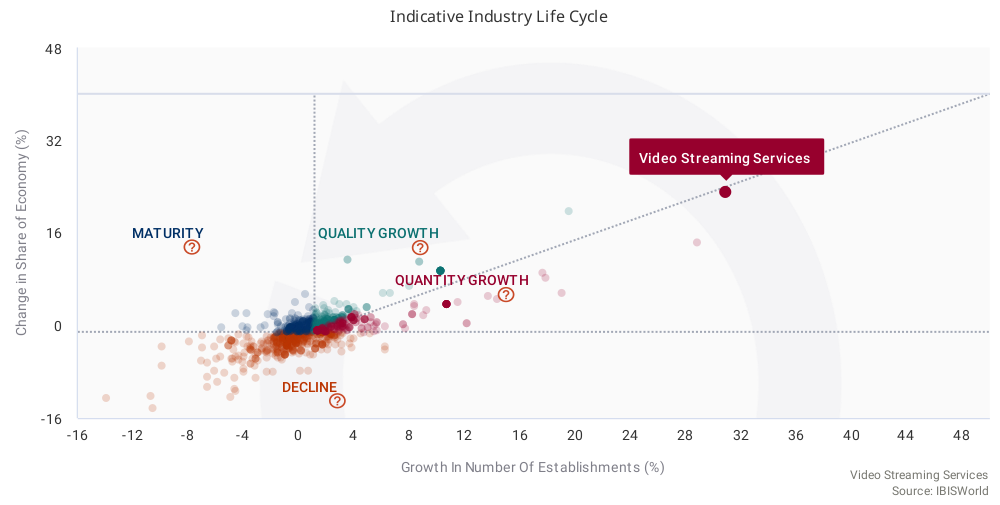
\includegraphics{Video_streaming_services_ibis.png}

The rapid expansion of this Video Streaming industry is cause for an
extensive analysis in factors leading to success in the market.

\begin{center}\rule{0.5\linewidth}{0.5pt}\end{center}

\hypertarget{assumptions}{%
\subsubsection{Assumptions}\label{assumptions}}

\begin{center}\rule{0.5\linewidth}{0.5pt}\end{center}

\begin{itemize}
\tightlist
\item
  While Hulu and Disney+ are both Disney owned companies, their
  streaming content differs, hence they will be treated individually.
\item
  Due to the fact that the latest release date in the dataset is in
  January, the following report assumes a data time-stamp of January
  2020
\item
  It is assumed that the dataset contains all titles listed/available on
  the streaming platform (ie. that it is exhaustive)
\item
  Age ratings are ``unrated'' if NA.
\item
  TV Shows data did not come with genre. Therefore the NA's were
  replaced with TV Show to get some insights from them anyway.
\end{itemize}

\begin{center}\rule{0.5\linewidth}{0.5pt}\end{center}

\hypertarget{research-questions}{%
\subsubsection{Research Questions}\label{research-questions}}

\begin{center}\rule{0.5\linewidth}{0.5pt}\end{center}

\begin{itemize}
\tightlist
\item
  Do some platforms host more of a certain genre or type than others?
\item
  Do all platforms have content of the same release years?
\item
  Which platform has the most exclusive content (not available on
  another platform)?
\item
  Does each streaming platform have a niche in terms of genre, age
  rating and type of content?
\item
  Do certain streaming platforms host better content than others?
\item
  What role does the streaming platform play on ratings?
\item
  Can Genre, streaming platform and release year be used to estimate a
  movie's IMDb rating?
\end{itemize}

\begin{center}\rule{0.5\linewidth}{0.5pt}\end{center}

\hypertarget{solving-the-problem}{%
\section{Solving the Problem}\label{solving-the-problem}}

\begin{center}\rule{0.5\linewidth}{0.5pt}\end{center}

\hypertarget{variable-selection}{%
\subsection{Variable Selection}\label{variable-selection}}

\begin{center}\rule{0.5\linewidth}{0.5pt}\end{center}

In order to answer the research questions, the analysis requires
information about the content hosted on popular streaming sites, such as
ratings, release dates, genre, type of content, and age rating. The main
data-set contains data relating to Netflix, Hulu, Disney+ and Prime
Video. There are several variables of metadata, as shown in the tibble
below.

\begin{Shaded}
\begin{Highlighting}[]
\NormalTok{variables }\OtherTok{\textless{}{-}} \FunctionTok{as\_tibble}\NormalTok{(}\FunctionTok{colnames}\NormalTok{(data\_movies\_tvshows))}

\CommentTok{\#printing dataset columns and their definitions}

\CommentTok{\# add a column describing the variable}
\NormalTok{variables}\SpecialCharTok{$}\NormalTok{Description }\OtherTok{\textless{}{-}} \FunctionTok{c}\NormalTok{(}\StringTok{"Title of Content"}\NormalTok{, }\StringTok{"Release year of content"}\NormalTok{, }\StringTok{"Age rating of content"}\NormalTok{, }\StringTok{"IMDb rating converted to 1{-}100"}\NormalTok{, }\StringTok{"Rotten Tomatoes Rating (1{-}100)"}\NormalTok{, }\StringTok{"Available on Netflix {-} Categorical Variable, (1=Yes)"}\NormalTok{,}\StringTok{"Available on hulu {-} Categorical Variable, (1=Yes)"}\NormalTok{,}\StringTok{"Available on prime video {-} Categorical Variable, (1=Yes)"}\NormalTok{,}\StringTok{"Available on Disney+ {-} Categorical Variable, (1=Yes)"}\NormalTok{,}\StringTok{" Categorical Variable, (1=TV{-}Series, 0=Movie)"}\NormalTok{,}\StringTok{"Names of directors"}\NormalTok{,}\StringTok{"Listed genres"}\NormalTok{, }\StringTok{"Countries of production"}\NormalTok{, }\StringTok{"Available languages"}\NormalTok{, }\StringTok{"runtime in minutes"}\NormalTok{, }\StringTok{"see year"}\NormalTok{, }\StringTok{"see disney+"}\NormalTok{, }\StringTok{"TV Show = True"}\NormalTok{)}
\NormalTok{variables }\SpecialCharTok{\%\textgreater{}\%} 
  \FunctionTok{rename}\NormalTok{(}\AttributeTok{Variable=}\StringTok{"value"}\NormalTok{)}\CommentTok{\#Renaming column names column to variables for readability}
\end{Highlighting}
\end{Shaded}

\begin{verbatim}
## # A tibble: 18 x 2
##    Variable        Description                                               
##    <chr>           <chr>                                                     
##  1 title           "Title of Content"                                        
##  2 year            "Release year of content"                                 
##  3 age             "Age rating of content"                                   
##  4 imdb            "IMDb rating converted to 1-100"                          
##  5 rotten_tomatoes "Rotten Tomatoes Rating (1-100)"                          
##  6 netflix         "Available on Netflix - Categorical Variable, (1=Yes)"    
##  7 hulu            "Available on hulu - Categorical Variable, (1=Yes)"       
##  8 prime_video     "Available on prime video - Categorical Variable, (1=Yes)"
##  9 disney+         "Available on Disney+ - Categorical Variable, (1=Yes)"    
## 10 type            " Categorical Variable, (1=TV-Series, 0=Movie)"           
## 11 directors       "Names of directors"                                      
## 12 genres          "Listed genres"                                           
## 13 country         "Countries of production"                                 
## 14 language        "Available languages"                                     
## 15 runtime         "runtime in minutes"                                      
## 16 release_year    "see year"                                                
## 17 disney          "see disney+"                                             
## 18 tvshow_or_movie "TV Show = True"
\end{verbatim}

\begin{center}\rule{0.5\linewidth}{0.5pt}\end{center}

\hypertarget{data-collection}{%
\subsection{Data Collection}\label{data-collection}}

\begin{center}\rule{0.5\linewidth}{0.5pt}\end{center}

The data-set that forms the basis of this analysis is a combination of 2
datasets from kaggle.com.\\
To extract as much information as possible, some mutations and data
cleaning was performed in the set-up chunk above. This includes renaming
certain columns, changing data from integers to logical and changing the
scale of the IMDb rating from 1-10 to 1-100 for better visualizations.\\
Furthermore, the data cleaning steps performed led to several subsets,
such as a tibble containing only titles that are hosted exclusively on
one platform, as well as titles that only belong to only one genre. The
exclusive platform dataset will be used for most visualizations in order
to compare the platforms on the basis of their exclusive content. Other
tibbles will be used for some visualizations to enhance comparison.\\
The data in some columns was deemed too complex to extract for the
purpose of this analysis. These included language, director and
country.\\
The genre column was however looked at, and titles that belonged to only
one genre were extracted to analyze trends across platforms.\\
Outliers, such as movies older than 70 years, and IMDb ratings = 0 were
filtered out of the dataset. The same applies to outlier titles with a
runtime in minutes below 10 minutes and above 250 minutes.\\
Several columns in the dataset include NA values, which were not removed
overall, due to the fact that some visualizations were reliant on data
in other columns.

\begin{center}\rule{0.5\linewidth}{0.5pt}\end{center}

\hypertarget{data-analysis}{%
\subsection{Data Analysis}\label{data-analysis}}

\begin{center}\rule{0.5\linewidth}{0.5pt}\end{center}

\hypertarget{prime-hosts-most-content-by-volume-hulus-content-majority-are-tv-shows}{%
\subsubsection{Prime hosts most content by Volume; Hulu's content
majority are TV
Shows}\label{prime-hosts-most-content-by-volume-hulus-content-majority-are-tv-shows}}

\begin{center}\rule{0.5\linewidth}{0.5pt}\end{center}

The first steps of this analysis aimed to learn more about the data, the
central tendencies, distributions, and counts. Amazon prime has by far
the most exclusive titles compared to any other platform. Disney+, as
the youngest platform of the comparison, has as expected, the least
number of exclusive titles. One possible explanation for the amount of
content via prime video is that the service offers some content as part
of its subscription and other titles on a pay per view (on-demand)
basis, which could skew the analysis in amazon's favor.\\
Overall, it is worth mentioning, that as a proportion, Hulu has more TV
shows, while all other platforms host more movies.

\begin{Shaded}
\begin{Highlighting}[]
\NormalTok{complete\_exclusive\_tibble }\SpecialCharTok{\%\textgreater{}\%}     \CommentTok{\#plotting movie proportions by streaming platform}
  \FunctionTok{group\_by}\NormalTok{(platform) }\SpecialCharTok{\%\textgreater{}\%}          \CommentTok{\#grouping by platform}
  \FunctionTok{count}\NormalTok{(tvshow\_or\_movie) }\SpecialCharTok{\%\textgreater{}\%}      \CommentTok{\#counting for the y axis}
  \FunctionTok{arrange}\NormalTok{(}\FunctionTok{desc}\NormalTok{(n)) }\SpecialCharTok{\%\textgreater{}\%}             \CommentTok{\#sorting from highest to lowest}
  \FunctionTok{ggplot}\NormalTok{(}\FunctionTok{aes}\NormalTok{(}\AttributeTok{x=}\NormalTok{ platform, }\AttributeTok{y=}\NormalTok{n))}\SpecialCharTok{+}  \CommentTok{\#adding titles}
  
  \CommentTok{\#adding a bar plot and dividing it by streaming platform}
  \FunctionTok{geom\_bar}\NormalTok{(}\FunctionTok{aes}\NormalTok{(}\AttributeTok{fill =}\NormalTok{tvshow\_or\_movie), }\AttributeTok{stat =} \StringTok{\textquotesingle{}identity\textquotesingle{}}\NormalTok{, }\AttributeTok{position=}\StringTok{"dodge"}\NormalTok{)}\SpecialCharTok{+}
  \CommentTok{\#adding title and changing axis labels}
  \FunctionTok{ggtitle}\NormalTok{(}\StringTok{"       TV Show : Movie Proportions by Streaming Service"}\NormalTok{) }\SpecialCharTok{+}
  \FunctionTok{xlab}\NormalTok{(}\StringTok{"Streaming Service"}\NormalTok{) }\SpecialCharTok{+} \FunctionTok{ylab}\NormalTok{(}\StringTok{"Number of Titles"}\NormalTok{)}\SpecialCharTok{+}
  \FunctionTok{scale\_fill\_manual}\NormalTok{(}\AttributeTok{name =} \StringTok{"Movie or TV Show"}\NormalTok{,}\AttributeTok{values=} \FunctionTok{c}\NormalTok{(}\StringTok{\textquotesingle{}navy\textquotesingle{}}\NormalTok{,}\StringTok{\textquotesingle{}brown\textquotesingle{}}\NormalTok{))}
\end{Highlighting}
\end{Shaded}

\includegraphics{Final_Team16_MsBA1_Mir_Wameling_files/figure-latex/Content Type and Volume by Platform-1.pdf}

\begin{center}\rule{0.5\linewidth}{0.5pt}\end{center}

\hypertarget{netflix-home-of-the-most-recent-titles-by-release-year}{%
\subsubsection{Netflix: home of the most recent titles by release
year}\label{netflix-home-of-the-most-recent-titles-by-release-year}}

\begin{center}\rule{0.5\linewidth}{0.5pt}\end{center}

The following boxplots revealed that the age of content on the four
different platforms varies quite significantly. While prime video
content spans the largest range with outliers as old as 100 years,
Netflix content is far more concentrated in recent years. This hints at
Netflix's strategy of producing a lot of proprietary content in large
volumes in the last 2 years (Business Insider, 2020).\\
The content on Hulu is similar in age (release\_year) as Netflix,
although not quite as concentrated. Disney+s' content is, as expected
nearly evenly distributed around the late nineties to early 2010s,
indicating its historically produced content, available on the service.

\begin{Shaded}
\begin{Highlighting}[]
\CommentTok{\#visualising the spread of the data by platform to see the age of their content}

\FunctionTok{ggplot}\NormalTok{(}\AttributeTok{data =}\NormalTok{ complete\_exclusive\_tibble,}\FunctionTok{aes}\NormalTok{(}\AttributeTok{y =}\NormalTok{ release\_year, }\AttributeTok{x =}\NormalTok{ platform, }\AttributeTok{color =}\NormalTok{ platform))}\SpecialCharTok{+}
  
  \CommentTok{\#adding jitter to have a sense of the number of titles offered by each platform}
  \FunctionTok{geom\_jitter}\NormalTok{(}\AttributeTok{alpha=}\FloatTok{0.1}\NormalTok{)}\SpecialCharTok{+}
  \FunctionTok{geom\_boxplot}\NormalTok{()}\SpecialCharTok{+}
  \CommentTok{\#correcting colours to match the color schemes of the streaming service logos}
  \FunctionTok{scale\_color\_manual}\NormalTok{(}\AttributeTok{name =} \StringTok{"Streaming Platform"}\NormalTok{,}\AttributeTok{values=} \FunctionTok{c}\NormalTok{(}\StringTok{\textquotesingle{}navy\textquotesingle{}}\NormalTok{,}\StringTok{\textquotesingle{}springgreen3\textquotesingle{}}\NormalTok{,}\StringTok{\textquotesingle{}red3\textquotesingle{}}\NormalTok{,}\StringTok{\textquotesingle{}darkturquoise\textquotesingle{}}\NormalTok{))}\SpecialCharTok{+}
  \FunctionTok{ggtitle}\NormalTok{(}\StringTok{"Release Year Distribution by Streaming Service}
\StringTok{+ added jitter layer to show the density of titles"}\NormalTok{) }\SpecialCharTok{+}
  \FunctionTok{xlab}\NormalTok{(}\StringTok{"Streaming Platform"}\NormalTok{) }\SpecialCharTok{+} \FunctionTok{ylab}\NormalTok{(}\StringTok{"Release Year of Content"}\NormalTok{)}
\end{Highlighting}
\end{Shaded}

\includegraphics{Final_Team16_MsBA1_Mir_Wameling_files/figure-latex/Release Year Distribution by Streaming Service-1.pdf}

\begin{center}\rule{0.5\linewidth}{0.5pt}\end{center}

\hypertarget{genres-and-platforms}{%
\subsubsection{Genres and platforms}\label{genres-and-platforms}}

\begin{center}\rule{0.5\linewidth}{0.5pt}\end{center}

The genre column was found to be cluttered with many concatenated genre
films/series. Therefore, an analysis looked at only the titles
containing a single genre. About 50\% of content falls into more than
one genre category (ie. ``Comedy,Drama''). The other half is primarily
made up of dramas and documentaries, closely followed by comedies. The
following graph shows the title count per genre and platform in
descending order of frequency. An overwhelming majority of titles fall
into the dramas and documentaries genre (n= 1245 and n=1077
respectively). This makes them the most frequent standalone genres and
Romance being the 9th most frequent, out of 25 genres with just 58
titles.

\begin{Shaded}
\begin{Highlighting}[]
\CommentTok{\# Showing volume of content available of streaming platforms by genre of content. }
\NormalTok{exclusive\_genre\_tibble }\SpecialCharTok{\%\textgreater{}\%} 
  \CommentTok{\#filtering the most popular genres we extracted during the EDA process}
  \FunctionTok{filter}\NormalTok{(genre\_1 }\SpecialCharTok{!=} \StringTok{\textquotesingle{}NA\textquotesingle{}} \SpecialCharTok{\&}\NormalTok{ genre\_1 }\SpecialCharTok{\%in\%} \FunctionTok{c}\NormalTok{(}\StringTok{\textquotesingle{}Drama\textquotesingle{}}\NormalTok{, }\StringTok{\textquotesingle{}Documentary\textquotesingle{}}\NormalTok{, }\StringTok{\textquotesingle{}Comedy\textquotesingle{}}\NormalTok{, }\StringTok{\textquotesingle{}Horror\textquotesingle{}}\NormalTok{, }\StringTok{\textquotesingle{}Thriller\textquotesingle{}}\NormalTok{, }\StringTok{"Action"}\NormalTok{, }\StringTok{"Western"}\NormalTok{, }\StringTok{"Family"}\NormalTok{,}\StringTok{"Romance"}\NormalTok{)) }\SpecialCharTok{\%\textgreater{}\%} 
  
  \FunctionTok{group\_by}\NormalTok{(platform) }\SpecialCharTok{\%\textgreater{}\%} 
  \FunctionTok{count}\NormalTok{(genre\_1) }\SpecialCharTok{\%\textgreater{}\%} 
  \FunctionTok{arrange}\NormalTok{(}\FunctionTok{desc}\NormalTok{(n)) }\SpecialCharTok{\%\textgreater{}\%} \CommentTok{\#sorting them in descending order}
  \FunctionTok{ggplot}\NormalTok{(}\FunctionTok{aes}\NormalTok{(}\FunctionTok{reorder}\NormalTok{( }\AttributeTok{x=}\NormalTok{ genre\_1, n), }\AttributeTok{y=}\NormalTok{n))}\SpecialCharTok{+}
  \CommentTok{\#plotting bar chart}
  \FunctionTok{geom\_bar}\NormalTok{(}\FunctionTok{aes}\NormalTok{(}\AttributeTok{fill =}\NormalTok{platform), }\AttributeTok{stat =} \StringTok{\textquotesingle{}identity\textquotesingle{}}\NormalTok{, }\AttributeTok{position =} \StringTok{\textquotesingle{}dodge\textquotesingle{}}\NormalTok{)}\SpecialCharTok{+}
  \FunctionTok{coord\_flip}\NormalTok{()}\SpecialCharTok{+} \CommentTok{\#flipping coordinates to incorporate to long texts of the genres}
  \CommentTok{\#filling colour according to official colours}
  \FunctionTok{scale\_fill\_manual}\NormalTok{(}\AttributeTok{name =} \StringTok{"Streaming Service"}\NormalTok{, }\AttributeTok{values=}\FunctionTok{c}\NormalTok{(}\StringTok{\textasciigrave{}}\AttributeTok{Disney+}\StringTok{\textasciigrave{}} \OtherTok{=} \StringTok{\textquotesingle{}navy\textquotesingle{}}\NormalTok{, }\StringTok{\textasciigrave{}}\AttributeTok{Hulu}\StringTok{\textasciigrave{}} \OtherTok{=} \StringTok{"springgreen3"}\NormalTok{, }\StringTok{\textasciigrave{}}\AttributeTok{Netflix}\StringTok{\textasciigrave{}} \OtherTok{=} \StringTok{"red3"}\NormalTok{, }\StringTok{\textasciigrave{}}\AttributeTok{Prime Video}\StringTok{\textasciigrave{}} \OtherTok{=} \StringTok{"darkturquoise"}\NormalTok{))}\SpecialCharTok{+}
  \FunctionTok{ggtitle}\NormalTok{(}\StringTok{"Top Genres by Streaming Platform"}\NormalTok{) }\SpecialCharTok{+}
  \FunctionTok{labs}\NormalTok{(}\AttributeTok{caption =} \StringTok{"TV Shows are excluded due to lack of Genre information"}\NormalTok{)}\SpecialCharTok{+}
  \FunctionTok{xlab}\NormalTok{(}\StringTok{"Genre"}\NormalTok{) }\SpecialCharTok{+} \FunctionTok{ylab}\NormalTok{(}\StringTok{"Number of Titles"}\NormalTok{)}
\end{Highlighting}
\end{Shaded}

\includegraphics{Final_Team16_MsBA1_Mir_Wameling_files/figure-latex/Genres and platforms-1.pdf}

The interesting thing about this is that a vast majority of content does
not fit into just one genre, but rather plays to multiple genres at
once. Typical combined titles were ``Comedy,Drama'' (n=446) and
``Drama,Romance'' (n=397), which could each potentially be boxed into a
genre on their own. This analysis refrained from doing so for the
purpose of this analysis.\\
It can further be noted that Disney+ is targeting the Family movies
niche and does not host any Horror, Thriller or Action content. Disney +
is however also hosting a relatively large proportion of Documentaries,
surprisingly.

\begin{center}\rule{0.5\linewidth}{0.5pt}\end{center}

\hypertarget{target-audience-of-platforms-according-to-age-ratings}{%
\subsubsection{Target Audience of Platforms according to Age
Ratings}\label{target-audience-of-platforms-according-to-age-ratings}}

\begin{center}\rule{0.5\linewidth}{0.5pt}\end{center}

\begin{Shaded}
\begin{Highlighting}[]
\CommentTok{\# Showing target audience by means of age ratings of content. }
\CommentTok{\#plotting a stacked barchart by genre and age rating}
\NormalTok{exclusive\_genre\_tibble }\SpecialCharTok{\%\textgreater{}\%} 
  \FunctionTok{filter}\NormalTok{(age}\SpecialCharTok{!=} \StringTok{"unrated"}\NormalTok{) }\SpecialCharTok{\%\textgreater{}\%} 
  \FunctionTok{group\_by}\NormalTok{(platform) }\SpecialCharTok{\%\textgreater{}\%} 
  \CommentTok{\# counting the number of titles belonging to an age rating level}
  \FunctionTok{count}\NormalTok{(age) }\SpecialCharTok{\%\textgreater{}\%} 
  \CommentTok{\# ordering the results by descending order}
  \FunctionTok{arrange}\NormalTok{(}\FunctionTok{desc}\NormalTok{(n)) }\SpecialCharTok{\%\textgreater{}\%} 
  \CommentTok{\# piping the result into a ggplot for visual analysis}
  \FunctionTok{ggplot}\NormalTok{(}\FunctionTok{aes}\NormalTok{(}\AttributeTok{x=}\NormalTok{ platform, }\AttributeTok{y=}\NormalTok{n))}\SpecialCharTok{+}
  \FunctionTok{geom\_bar}\NormalTok{(}\FunctionTok{aes}\NormalTok{(}\AttributeTok{fill =}\NormalTok{age), }
           \CommentTok{\# creating a stacked bar chart with fill equal to the age rating}
           \AttributeTok{stat =} \StringTok{\textquotesingle{}identity\textquotesingle{}}\NormalTok{, }
           \AttributeTok{position =} \StringTok{"fill"}\NormalTok{)}\SpecialCharTok{+}
  \CommentTok{\#adding labels to the graph}
  \FunctionTok{ggtitle}\NormalTok{(}\StringTok{"Proportions of Various Age restrictions}\SpecialCharTok{\textbackslash{}n}\StringTok{by Streaming Service"}\NormalTok{) }\SpecialCharTok{+}
  \FunctionTok{xlab}\NormalTok{(}\StringTok{"Streaming Service"}\NormalTok{) }\SpecialCharTok{+} 
  \FunctionTok{ylab}\NormalTok{(}\StringTok{"Relative Frequency"}\NormalTok{)}\SpecialCharTok{+}
  \FunctionTok{scale\_fill\_manual}\NormalTok{(}\AttributeTok{name =} \StringTok{"Age Rating"}\NormalTok{,}
                    \AttributeTok{values =} \FunctionTok{c}\NormalTok{(}\StringTok{"13+"}\OtherTok{=}\StringTok{"purple3"}\NormalTok{, }
                               \StringTok{\textquotesingle{}16+\textquotesingle{}}\OtherTok{=}\StringTok{"orange"}\NormalTok{, }
                               \StringTok{\textquotesingle{}18+\textquotesingle{}}\OtherTok{=}\StringTok{"black"}\NormalTok{, }
                               \StringTok{\textquotesingle{}7+\textquotesingle{}}\OtherTok{=}\StringTok{"lightblue"}\NormalTok{, }
                               \StringTok{\textquotesingle{}all\textquotesingle{}}\OtherTok{=}\StringTok{"pink3"}\NormalTok{))}\SpecialCharTok{+}
  \FunctionTok{ggtitle}\NormalTok{(}\StringTok{"Popular Genre Proportions }\SpecialCharTok{\textbackslash{}n}\StringTok{by Streaming Service"}\NormalTok{) }\SpecialCharTok{+}
  \FunctionTok{xlab}\NormalTok{(}\StringTok{"Genre"}\NormalTok{) }\SpecialCharTok{+} 
  \FunctionTok{ylab}\NormalTok{(}\StringTok{"Relative Frequency"}\NormalTok{)}
\end{Highlighting}
\end{Shaded}

\includegraphics{Final_Team16_MsBA1_Mir_Wameling_files/figure-latex/Target Audience acording to age ratings-1.pdf}

It is evident that Disney targets a completely different audience, with
large majority of content available being aimed at all ages and children
aged 7 and over. The other platforms have less emphasis on those age
ratings, but rather on the content available for ages 16+. What is
excluded from this visual is the volume of content that remains unrated,
as one can only assume what ``unrated'' means in each case. For some
titles this might mean more brutality for others this might just mean
that the movie/series was not produced for TV and hence never received a
rating. The best place to go for a broad range of content seems to be
Amazon Prime, although the bias of paid content potentially being
included in the dataset remains.

\begin{center}\rule{0.5\linewidth}{0.5pt}\end{center}

\hypertarget{distribution-of-imdb-ratings}{%
\subsubsection{Distribution of IMDb
ratings}\label{distribution-of-imdb-ratings}}

\begin{center}\rule{0.5\linewidth}{0.5pt}\end{center}

After running basic summary functions, the analysis looked at the IMDb
ratings of content exclusively available on any of the platforms, where
available. All distributions of ratings resemble normal or near-normal
distribution with slight skewness to the left.

It seems amazon prime video content has the lowest mean IMDB rating and
the broadest distribution. Hulu's content is rated the highest on
average from all the platforms in this dataset. Disney+ and Netflix are
somewhere in the middle, quite close together.

\begin{Shaded}
\begin{Highlighting}[]
\CommentTok{\#plotting a density plot to show the number of titles offered by the different platforms, their spread over the imdb ratings and their respective medians.}

\NormalTok{complete\_exclusive\_tibble }\SpecialCharTok{\%\textgreater{}\%} 
  \FunctionTok{filter}\NormalTok{(imdb }\SpecialCharTok{!=} \StringTok{\textquotesingle{}NA\textquotesingle{}}\NormalTok{) }\SpecialCharTok{\%\textgreater{}\%} \CommentTok{\#removing NA\textquotesingle{}s}
  \FunctionTok{group\_by}\NormalTok{(platform) }\SpecialCharTok{\%\textgreater{}\%} 
  \FunctionTok{count}\NormalTok{(imdb) }\SpecialCharTok{\%\textgreater{}\%} 
  \FunctionTok{arrange}\NormalTok{(}\FunctionTok{desc}\NormalTok{(n)) }\SpecialCharTok{\%\textgreater{}\%} 
  \FunctionTok{ggplot}\NormalTok{(}\FunctionTok{aes}\NormalTok{(}\AttributeTok{x=}\NormalTok{ imdb, }\AttributeTok{y=}\NormalTok{n))}\SpecialCharTok{+}
  
  \CommentTok{\#plotting the medians}
  \FunctionTok{geom\_vline}\NormalTok{(}\FunctionTok{aes}\NormalTok{(}\AttributeTok{xintercept =} \FunctionTok{median}\NormalTok{(prime\_video\_exclusive\_tibble}\SpecialCharTok{$}\NormalTok{imdb,}\AttributeTok{na.rm =} \ConstantTok{TRUE}\NormalTok{)),}
             \AttributeTok{color=}\StringTok{\textquotesingle{}darkturquoise\textquotesingle{}}\NormalTok{,}
             \AttributeTok{size=}\DecValTok{1}\NormalTok{)}\SpecialCharTok{+}
  \FunctionTok{geom\_vline}\NormalTok{(}\FunctionTok{aes}\NormalTok{(}\AttributeTok{xintercept =} \FunctionTok{median}\NormalTok{(netflix\_exclusive\_tibble}\SpecialCharTok{$}\NormalTok{imdb,}\AttributeTok{na.rm =} \ConstantTok{TRUE}\NormalTok{)),}
           \AttributeTok{color=}\StringTok{\textquotesingle{}red3\textquotesingle{}}\NormalTok{,}
           \AttributeTok{size=}\DecValTok{1}\NormalTok{)}\SpecialCharTok{+}
  \FunctionTok{geom\_vline}\NormalTok{(}\FunctionTok{aes}\NormalTok{(}\AttributeTok{xintercept =} \FunctionTok{median}\NormalTok{(hulu\_exclusive\_tibble}\SpecialCharTok{$}\NormalTok{imdb,}\AttributeTok{na.rm =} \ConstantTok{TRUE}\NormalTok{)),}
           \AttributeTok{color=}\StringTok{\textquotesingle{}springgreen3\textquotesingle{}}\NormalTok{,}
           \AttributeTok{size=}\DecValTok{1}\NormalTok{)}\SpecialCharTok{+}
  \FunctionTok{geom\_vline}\NormalTok{(}\FunctionTok{aes}\NormalTok{(}\AttributeTok{xintercept =} \FunctionTok{median}\NormalTok{(disney\_exclusive\_tibble}\SpecialCharTok{$}\NormalTok{imdb,}\AttributeTok{na.rm =} \ConstantTok{TRUE}\NormalTok{)),}
           \AttributeTok{color=}\StringTok{\textquotesingle{}navy\textquotesingle{}}\NormalTok{,}
           \AttributeTok{size=}\DecValTok{1}\NormalTok{)}\SpecialCharTok{+}
  
  \CommentTok{\#titles and axis labelling}
  \FunctionTok{ggtitle}\NormalTok{(}\StringTok{"IMDb Rating Distributions by Streaming Service"}\NormalTok{)}\SpecialCharTok{+}
  \FunctionTok{labs}\NormalTok{(}\AttributeTok{caption =} \StringTok{"Amazon has most content, Hulu has highest average IMDb ratings"}\NormalTok{) }\SpecialCharTok{+}
  \FunctionTok{xlab}\NormalTok{(}\StringTok{"IMDb Rating"}\NormalTok{) }\SpecialCharTok{+} \FunctionTok{ylab}\NormalTok{(}\StringTok{"Frequency"}\NormalTok{)}\SpecialCharTok{+}
  
  \CommentTok{\#density plot and platforms\textquotesingle{} respective colors}
  \FunctionTok{geom\_density}\NormalTok{(}\FunctionTok{aes}\NormalTok{(}\AttributeTok{fill =}\NormalTok{platform),}\AttributeTok{alpha=}\FloatTok{0.5}\NormalTok{,  }\AttributeTok{stat =} \StringTok{\textquotesingle{}identity\textquotesingle{}}\NormalTok{, }\AttributeTok{position =} \StringTok{\textquotesingle{}dodge\textquotesingle{}}\NormalTok{)}\SpecialCharTok{+}
  \FunctionTok{scale\_fill\_manual}\NormalTok{(}\AttributeTok{name =} \StringTok{"Streaming Service"}\NormalTok{,}\AttributeTok{values=} \FunctionTok{c}\NormalTok{(}\StringTok{\textquotesingle{}navy\textquotesingle{}}\NormalTok{,}\StringTok{\textquotesingle{}springgreen3\textquotesingle{}}\NormalTok{,}\StringTok{\textquotesingle{}red3\textquotesingle{}}\NormalTok{,}\StringTok{\textquotesingle{}darkturquoise\textquotesingle{}}\NormalTok{))}
\end{Highlighting}
\end{Shaded}

\includegraphics{Final_Team16_MsBA1_Mir_Wameling_files/figure-latex/IMDb ratings distributions and mean ratings-1.pdf}

The analysis continued to look at trends within the rating of films over
time (release\_year) to see if older or newer titles resonated better
with the general public.

\begin{center}\rule{0.5\linewidth}{0.5pt}\end{center}

\hypertarget{older-titles-are-on-average-better-rated-than-newer-content.}{%
\subsubsection{Older titles are on average better rated than newer
content.}\label{older-titles-are-on-average-better-rated-than-newer-content.}}

\begin{center}\rule{0.5\linewidth}{0.5pt}\end{center}

\begin{Shaded}
\begin{Highlighting}[]
\CommentTok{\# release year v rating}
\CommentTok{\#plotting geom\_smooth regressions to see the trends of the platforms imdb ratings over time}
\NormalTok{complete\_exclusive\_tibble }\SpecialCharTok{\%\textgreater{}\%} 
  \CommentTok{\#keeping the last 2 decades, to not let outliers bias our results}
  \FunctionTok{filter}\NormalTok{(release\_year }\SpecialCharTok{\textgreater{}} \DecValTok{2000}\NormalTok{) }\SpecialCharTok{\%\textgreater{}\%}  
  \FunctionTok{ggplot}\NormalTok{(}\FunctionTok{aes}\NormalTok{(}
    \AttributeTok{y =}\NormalTok{ imdb, }
    \AttributeTok{x =}\NormalTok{ release\_year, }
    \AttributeTok{color =}\NormalTok{ platform) , }
    \AttributeTok{alpha=}\FloatTok{0.05}\NormalTok{)}\SpecialCharTok{+}
  \CommentTok{\#using linear models for linear comparisons}
  \FunctionTok{geom\_smooth}\NormalTok{(}\AttributeTok{method =} \StringTok{\textquotesingle{}lm\textquotesingle{}}\NormalTok{)}\SpecialCharTok{+}
  \CommentTok{\# setting custom colors and labels}
  \FunctionTok{scale\_color\_manual}\NormalTok{(}
    \AttributeTok{name =} \StringTok{"Streaming Service"}\NormalTok{,}
    \AttributeTok{values=} \FunctionTok{c}\NormalTok{(}\StringTok{\textquotesingle{}navy\textquotesingle{}}\NormalTok{,}\StringTok{\textquotesingle{}springgreen3\textquotesingle{}}\NormalTok{,}\StringTok{\textquotesingle{}red3\textquotesingle{}}\NormalTok{,}\StringTok{\textquotesingle{}darkturquoise\textquotesingle{}}\NormalTok{)) }\SpecialCharTok{+}
  \FunctionTok{ggtitle}\NormalTok{(}\StringTok{"Plots of Linear Regressions of }\SpecialCharTok{\textbackslash{}n}\StringTok{IMDb Ratings Against Release Year"}\NormalTok{) }\SpecialCharTok{+}
  \FunctionTok{xlab}\NormalTok{(}\StringTok{"Release Year"}\NormalTok{) }\SpecialCharTok{+} 
  \FunctionTok{ylab}\NormalTok{(}\StringTok{"IMDb Rating"}\NormalTok{)}
\end{Highlighting}
\end{Shaded}

\includegraphics{Final_Team16_MsBA1_Mir_Wameling_files/figure-latex/Release Year versus IMDb Rating-1.pdf}
As evident from the graph, newer Disney + content is rated much higher
than older Disney + content. The opposite is true for content hosted on
Amazon Prime Video, Netflix and Hulu. The error zones are quite large on
most of the best-fit lines, but the trends are undeniable. Release year
seems to play a role in IMDb rating.

\begin{center}\rule{0.5\linewidth}{0.5pt}\end{center}

\hypertarget{outliers-natural-language-variables}{%
\subsubsection{Outliers \& Natural Language
Variables}\label{outliers-natural-language-variables}}

\begin{center}\rule{0.5\linewidth}{0.5pt}\end{center}

The analysis looked at numerical variables and simpler categorical
variables to judge the quality of the content on each platform. The
analysis revealed that nearly 70\% of titles did not have a rotten
tomato score and hence the IMDb rating was considered the best judge of
quality in this analysis. This is further supported by the fact how
these ratings are generated. While Rotten Tomatoes Scores are based on
critics' reviews, IMDb ratings are contributed by the general public
(Colbert, 2017). The validity of those scores in this analysis stems
from the fact that the general public will be the paying customer for
any viewing platform.\\
Furthermore, several columns were not taken into consideration, as their
content was too complex to prepare it for inclusion to linear models.\\
While initially, the analysis aimed to explain why a certain title of
content would be hosted on a particular platform, the direction shifted
into an inference model of IMDb rating based on several parameters.\\
Although the initial linear model of formula= netflix \textasciitilde{}
imdb + year resulted in a 0.1 = r-squared, hinted at a possible
connection between platform, IMDb scores, and release year, the model
could not be improved due to lack of additional data.

\begin{center}\rule{0.5\linewidth}{0.5pt}\end{center}

\hypertarget{stating-the-hypothesis}{%
\subsection{Stating the Hypothesis}\label{stating-the-hypothesis}}

\begin{center}\rule{0.5\linewidth}{0.5pt}\end{center}

After studying all the relationships within the data the analysis
shifted, to explain the IMDb rating by means of several variables. \[
\begin{aligned}
H_0 &: \text{ The provided variables do not aid in explaining a titles’ IMDb score. } (r^2 =0) \\
H_A &: \text{ The model is able to explain the IMDb score to some extent. }(r^2 >0)
\end{aligned}
\]

The alternative hypothesis is that our model can explain the IMDb score
of a movie or TV show, given its release year, genre, age rating and the
platform where it is hosted.

\begin{center}\rule{0.5\linewidth}{0.5pt}\end{center}

\hypertarget{modelling-and-comunication}{%
\section{Modelling and Comunication}\label{modelling-and-comunication}}

\begin{center}\rule{0.5\linewidth}{0.5pt}\end{center}

As the preceding analysis section revealed, there were some stronger and
weaker indicators for IMDb rating across the different variables in this
TV Show and Movies dataset. What remains true, is that there are still
lurking variables, when trying to explain the IMDb score, which are not
available in the following model.\\
However, there is strong evidence to reject the null hypothesis, that
there is no way to explain a titles' IMDb rating given the available
information.

\begin{center}\rule{0.5\linewidth}{0.5pt}\end{center}

\hypertarget{modelling}{%
\subsection{Modelling}\label{modelling}}

\begin{center}\rule{0.5\linewidth}{0.5pt}\end{center}

The most promising regression model built is based on the following
formula:

\[
\text{IMDb} = f(\text{ TV show or Movie+ Genre + Release Year + Age Rating  + Streaming Platform})
\]

IMDb scores are a function of content type, controlling for Genre,
Release Year, Age Rating and Streaming platform.

\begin{Shaded}
\begin{Highlighting}[]
\CommentTok{\# building a model to explain IMDb rating based on 5 variables and several levels}
\NormalTok{regression\_model}\OtherTok{\textless{}{-}}\FunctionTok{lm}\NormalTok{(}
  \AttributeTok{formula =}\NormalTok{ imdb }\SpecialCharTok{\textasciitilde{}}\NormalTok{ tvshow\_or\_movie }
  \SpecialCharTok{+}\NormalTok{ year }
  \SpecialCharTok{+}\NormalTok{ age }
  \SpecialCharTok{+}\NormalTok{ platform}
  \SpecialCharTok{+}\NormalTok{ genre\_1, }
  \AttributeTok{data=}\NormalTok{exclusive\_genre\_tibble)}

\CommentTok{\# Summarizing the output of the model using the broom library}
\NormalTok{broom}\SpecialCharTok{::}\FunctionTok{glance}\NormalTok{(regression\_model)}
\end{Highlighting}
\end{Shaded}

\begin{verbatim}
## # A tibble: 1 x 12
##   r.squared adj.r.squared sigma statistic p.value    df  logLik    AIC    BIC
##       <dbl>         <dbl> <dbl>     <dbl>   <dbl> <dbl>   <dbl>  <dbl>  <dbl>
## 1     0.355         0.353  11.2      138.       0    35 -33626. 67326. 67588.
## # ... with 3 more variables: deviance <dbl>, df.residual <int>, nobs <int>
\end{verbatim}

\begin{Shaded}
\begin{Highlighting}[]
\NormalTok{broom}\SpecialCharTok{::}\FunctionTok{tidy}\NormalTok{(regression\_model)}
\end{Highlighting}
\end{Shaded}

\begin{verbatim}
## # A tibble: 37 x 5
##    term                   estimate std.error statistic   p.value
##    <chr>                     <dbl>     <dbl>     <dbl>     <dbl>
##  1 (Intercept)           51.8      1.49         34.8   2.95e-248
##  2 tvshow_or_movietvshow 22.8      0.985        23.1   1.49e-114
##  3 year                  -0.000214 0.0000245    -8.74  2.78e- 18
##  4 age16+                 1.07     0.829         1.30  1.95e-  1
##  5 age18+                 0.404    0.778         0.520 6.03e-  1
##  6 age7+                 -0.792    0.812        -0.976 3.29e-  1
##  7 ageall                -2.28     0.882        -2.59  9.57e-  3
##  8 ageunrated            -0.619    0.733        -0.844 3.99e-  1
##  9 platformHulu          -1.31     0.882        -1.49  1.37e-  1
## 10 platformNetflix        1.49     0.860         1.73  8.29e-  2
## # ... with 27 more rows
\end{verbatim}

The overall explanatory power of the model is above 35\% and the p-value
of \textless{} 0.00 indicates that this is not likely due to chance.
Hence, we can reject the \(H_0\) and say that the effect is
\emph{statistically significant}. In essence, the model helps to explain
the IMDb rating a title has received by the voting population on IMDb.
Outright, this includes the average attractiveness of a genre, type,
release year, age rating and streaming platform over another.

\begin{center}\rule{0.5\linewidth}{0.5pt}\end{center}

\hypertarget{results-presentation}{%
\subsection{Results Presentation}\label{results-presentation}}

\begin{center}\rule{0.5\linewidth}{0.5pt}\end{center}

There are particular coefficients and genres that stuck out, which tie
back into the earlier analysis. When looking at the p-value, for release
year, it confirms the earlier visible trends in IMDb ratings declining
in recent years. The coefficient for release year is also negative.
There are a few other coefficients which support the earlier analysis,
such as the coefficients for genre = Family, Drama and Documentary. All
of these p-values are very low and add to the explanatory power of this
model, given that a title falls into one of these categories.

The \(r^2\) of this model at 35\% is quite strong, but it does, also
raise new questions about other factors that influence the preferences
of people voting on IMDb. The following list is just an excerpt of the
potential lurking variables that come to mind, which if answered could
help to better explain the IMDb rating.

\begin{itemize}
\tightlist
\item
  How many IMDb votes did the title receive?
\item
  What gender were the viewers and voters of the content? Are they the
  same people or did parents vote for the content their children
  watched?
\item
  How many people watched a title?
\item
  Where are the viewers and voters from geographically?
\item
  What country was the content produced in?
\item
  What kind of budget was spent on marketing the content to the
  audience?
\end{itemize}

\begin{center}\rule{0.5\linewidth}{0.5pt}\end{center}

\hypertarget{key-takeaways}{%
\subsection{Key Takeaways}\label{key-takeaways}}

\begin{center}\rule{0.5\linewidth}{0.5pt}\end{center}

Given the limitations of the dataset possible, as much information as
was possible was extracted to build the above model. Most research
questions could be answered and clear trends were identified.

\begin{itemize}
\tightlist
\item
  Some platforms target their audience with a specific genre, others
  with a specific type of content and age rating.\\
\item
  Amazon Prime Video has the widest variety of content available among
  all investigated platforms.\\
\item
  The IMDb ratings are normally distributed, therefore we can rely on
  their central tendency and hazard a statement that on average Hulu
  hosts the best content, followed by Netflix and Disney+
\end{itemize}

\begin{center}\rule{0.5\linewidth}{0.5pt}\end{center}

\hypertarget{suggestions-for-further-research-and-analysis}{%
\subsection{Suggestions for further Research and
Analysis}\label{suggestions-for-further-research-and-analysis}}

\begin{center}\rule{0.5\linewidth}{0.5pt}\end{center}

The analysis was not able to identify a clearly defined niche for a
new-entrant, but there is plenty of opportunity given the projected
growth in the market overall.

Supplementary data would be needed to answer the newly raised questions,
to better explain IMDb ratings and learn more about the voters'
preferences leading to higher or lower ratings. Furthmore, it would add
an additional layer of insight if this qualitative analysis was merged
with a financial impact analysis. This could reveal a potentially
lucrative niche among on-demand video hosting platforms.

\begin{center}\rule{0.5\linewidth}{0.5pt}\end{center}

\hypertarget{sources}{%
\section{Sources}\label{sources}}

\begin{center}\rule{0.5\linewidth}{0.5pt}\end{center}

Bhatia, R. (2020, January). Movies on Netflix, Prime Video, Hulu and
Disney+. From Kaggle.com:
\href{https://www.kaggle.com/ruchi798/movies-on-netflix-prime-video-hulu-and-disney}{Kaggle.com}

Bhatia, R. (2020, January). TV shows on Netflix, Prime Video, Hulu and
Disney+. From Kaggle.com:
\href{https://www.kaggle.com/ruchi798/tv-shows-on-netflix-prime-video-hulu-and-disney}{Kaggle.com}

Watson, A. (2020, October 21). Netflix's revenue Q1 2011-Q3 2020. From
Statista:
\href{https://www.statista.com/statistics/273883/netflixs-quarterly-revenue/}{Statista.com}

Graham, J. (2020, January). Disney+ already tops 40 million subscriber,
a quarter of Netflix audience, report says. From USA Today:
\href{https://www.usatoday.com/story/tech/2020/01/15/disney-has-over-40-m-subscribers-1-4-size-netflix-2-months/4469107002/}{USA
Today}

Cook, D. (2020, November). Video Streaming Services in the US. From IBIS
World:
\href{https://my-ibisworld-com.hult.idm.oclc.org/us/en/industry-specialized/od6197/competitive-landscape}{Ibis
World}

Colbert, S. M. (2017, September). Rotten Tomatoes, Metacritic, IMDb \&
CinemaScore Explained. From ScreenRant:
\href{https://screenrant.com/rotten-tomatoes-metacritic-imdb-cinemascore-explained/}{Screen
Rant}

Clark, T. (2020, January). We compared what the 6 major streaming TV
services offer, from Netflix to Disney Plus to Hulu. From Business
Insider:
\href{https://www.businessinsider.com/streaming-comparison-netflix-disney-plus-hulu-prime-video-2020-1}{Business
Insider}

\end{document}
